%  Field_Modelling.tex
% !TeX spellcheck = en_GB
% !TeX root = ReportMain.tex

\section{Modelling Results}
The following simulations were completed using the COMSOL multiphysics software package.
COMSOL is a professional finite element simulation package able to model a variety of physical features.
The following models are created using the AC/DC module, which is used to simulate electric and magnetic fields \cite{ACDCCOMSOLMODULE}.
Specifically, the electrostatics interface is used. 
This solves a charge conservation equation for a given voltage and spacial distribution of charge.

The charge conservation equation is:
\begin{equation}
E = -\nabla V
\end{equation}

The equations are derived from Maxwell's equations 

\subsection{Workflow}
In order to simulate the electric field distribution within our bushing design, 2D axisymmetric models were created. The general workflow to achieve this is:
\begin{enumerate}
\item Build a geometry representing the physical structure of the bushing.
\item Assign each geometric domain a material. The material selection determines the relative permittivity $\epsilon_r$ of each domain.
\item Define the charge conservation equation and all initial conditions. This includes setting which boundaries are at ground and conductor potential and setting boundary conditions.
\item Design a mesh. The geometry is split into smaller elements in order to compute the charge conservation equation. For designs with foils, special meshing parameters are required to speed up the process.
\item Carry out the study. This stage is the actual computation of the solution.
\item Post-processing - Display the results in a number of formats including 3D, 2D and 1D plots, or export the data for post-processing in Matlab.
\end{enumerate}


\subsection{Baseline Model}
In order to minimise the computation time required for each model, it was necessary to determine the areas of interest in the model.
A bushing geometry was built with no foils inserted, a high quality mesh was produced and the system was solved to find the electric field distribution throughout the bushing and the surrounding area.
\begin{figure}[!htb]
  \centering
  \subfigure[Geometry]{
    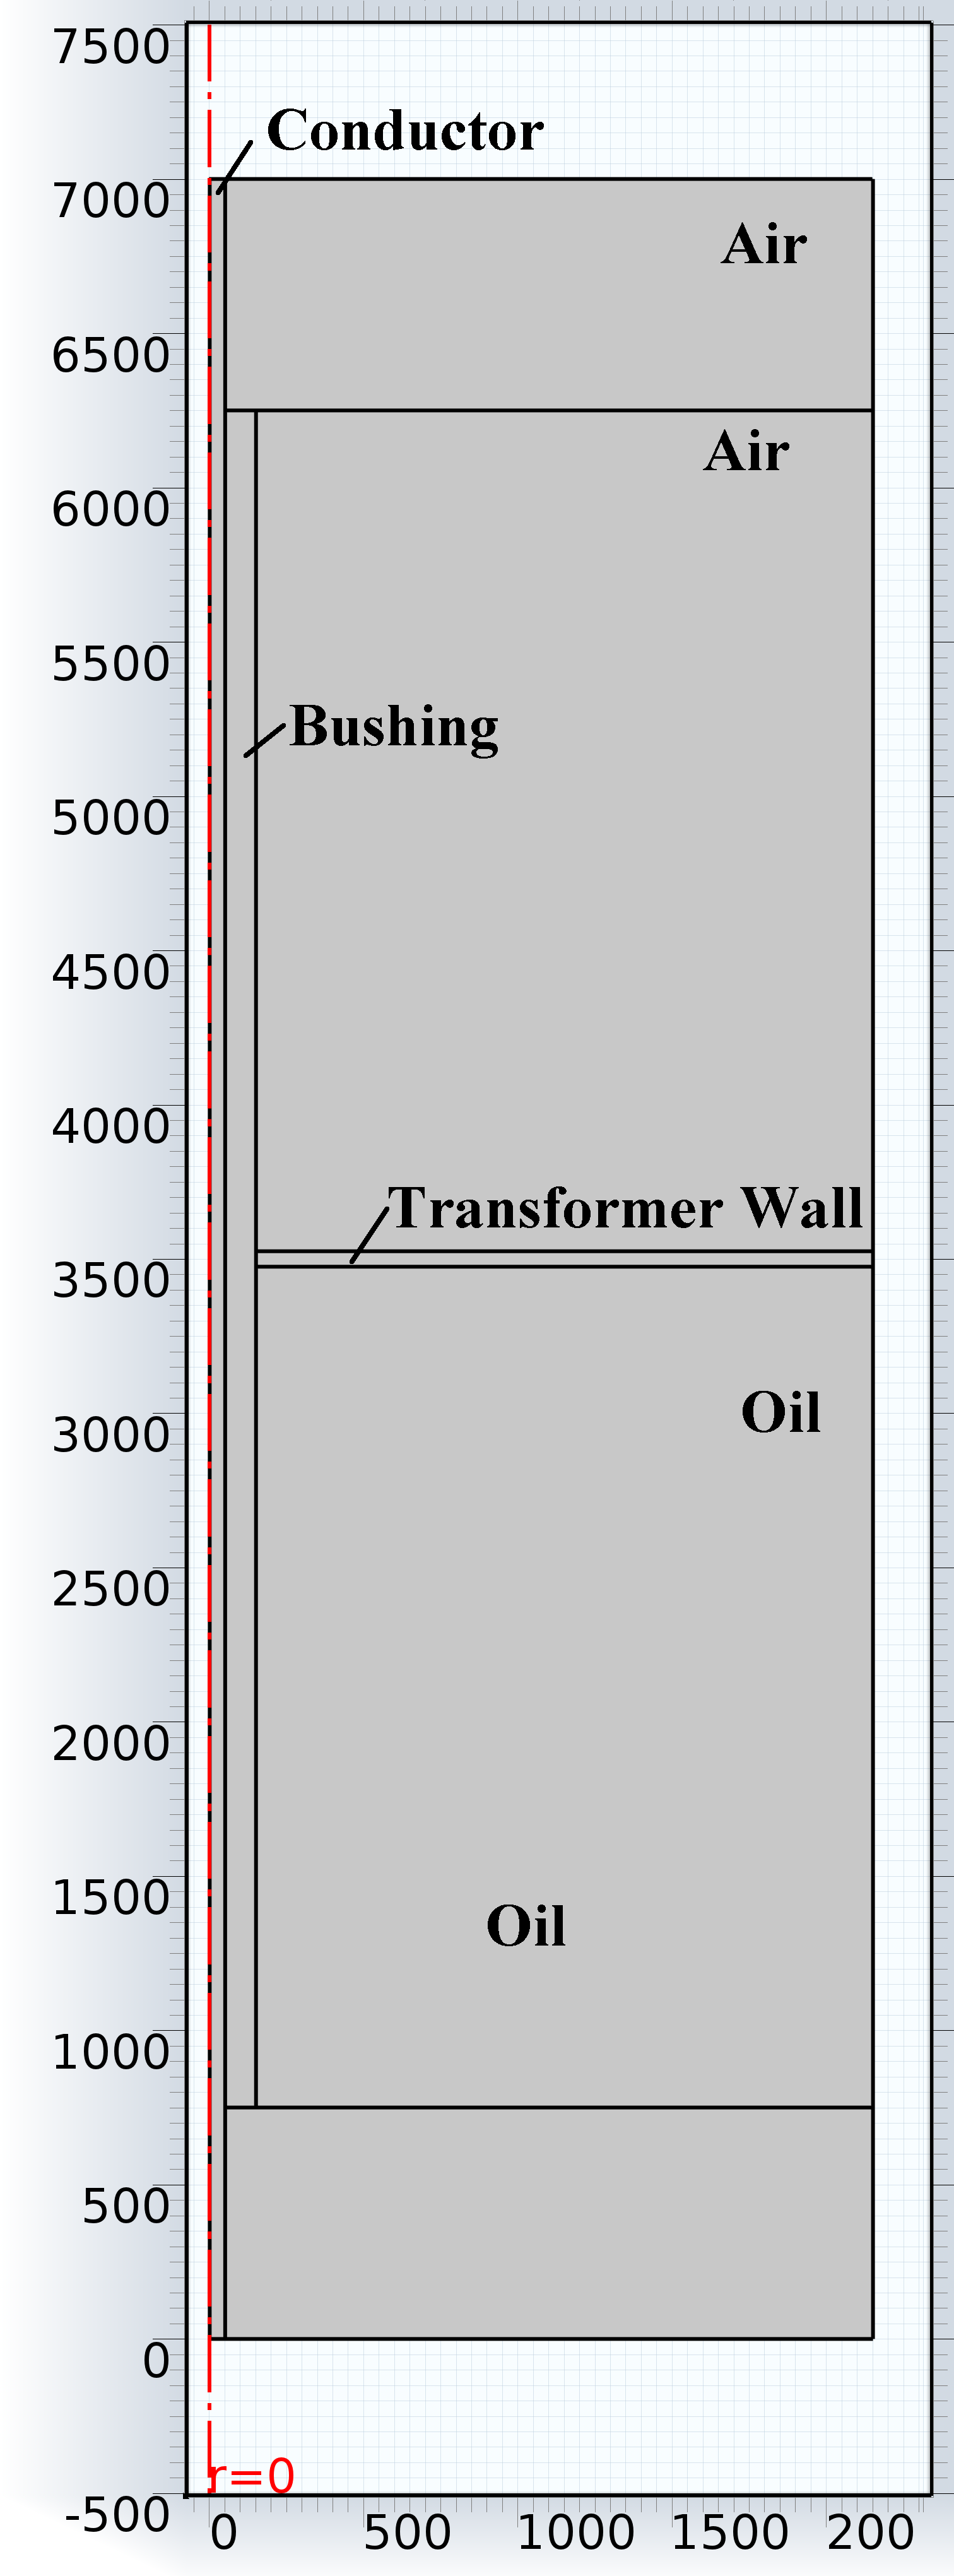
\includegraphics[height = 10cm]{./Figures/Simulations/Edited_No_Foils_Large/Geometry.png} 
	\label{Figure:No_Foil_Large_Geom}
  }
  \subfigure[Extra Fine Mesh]{
    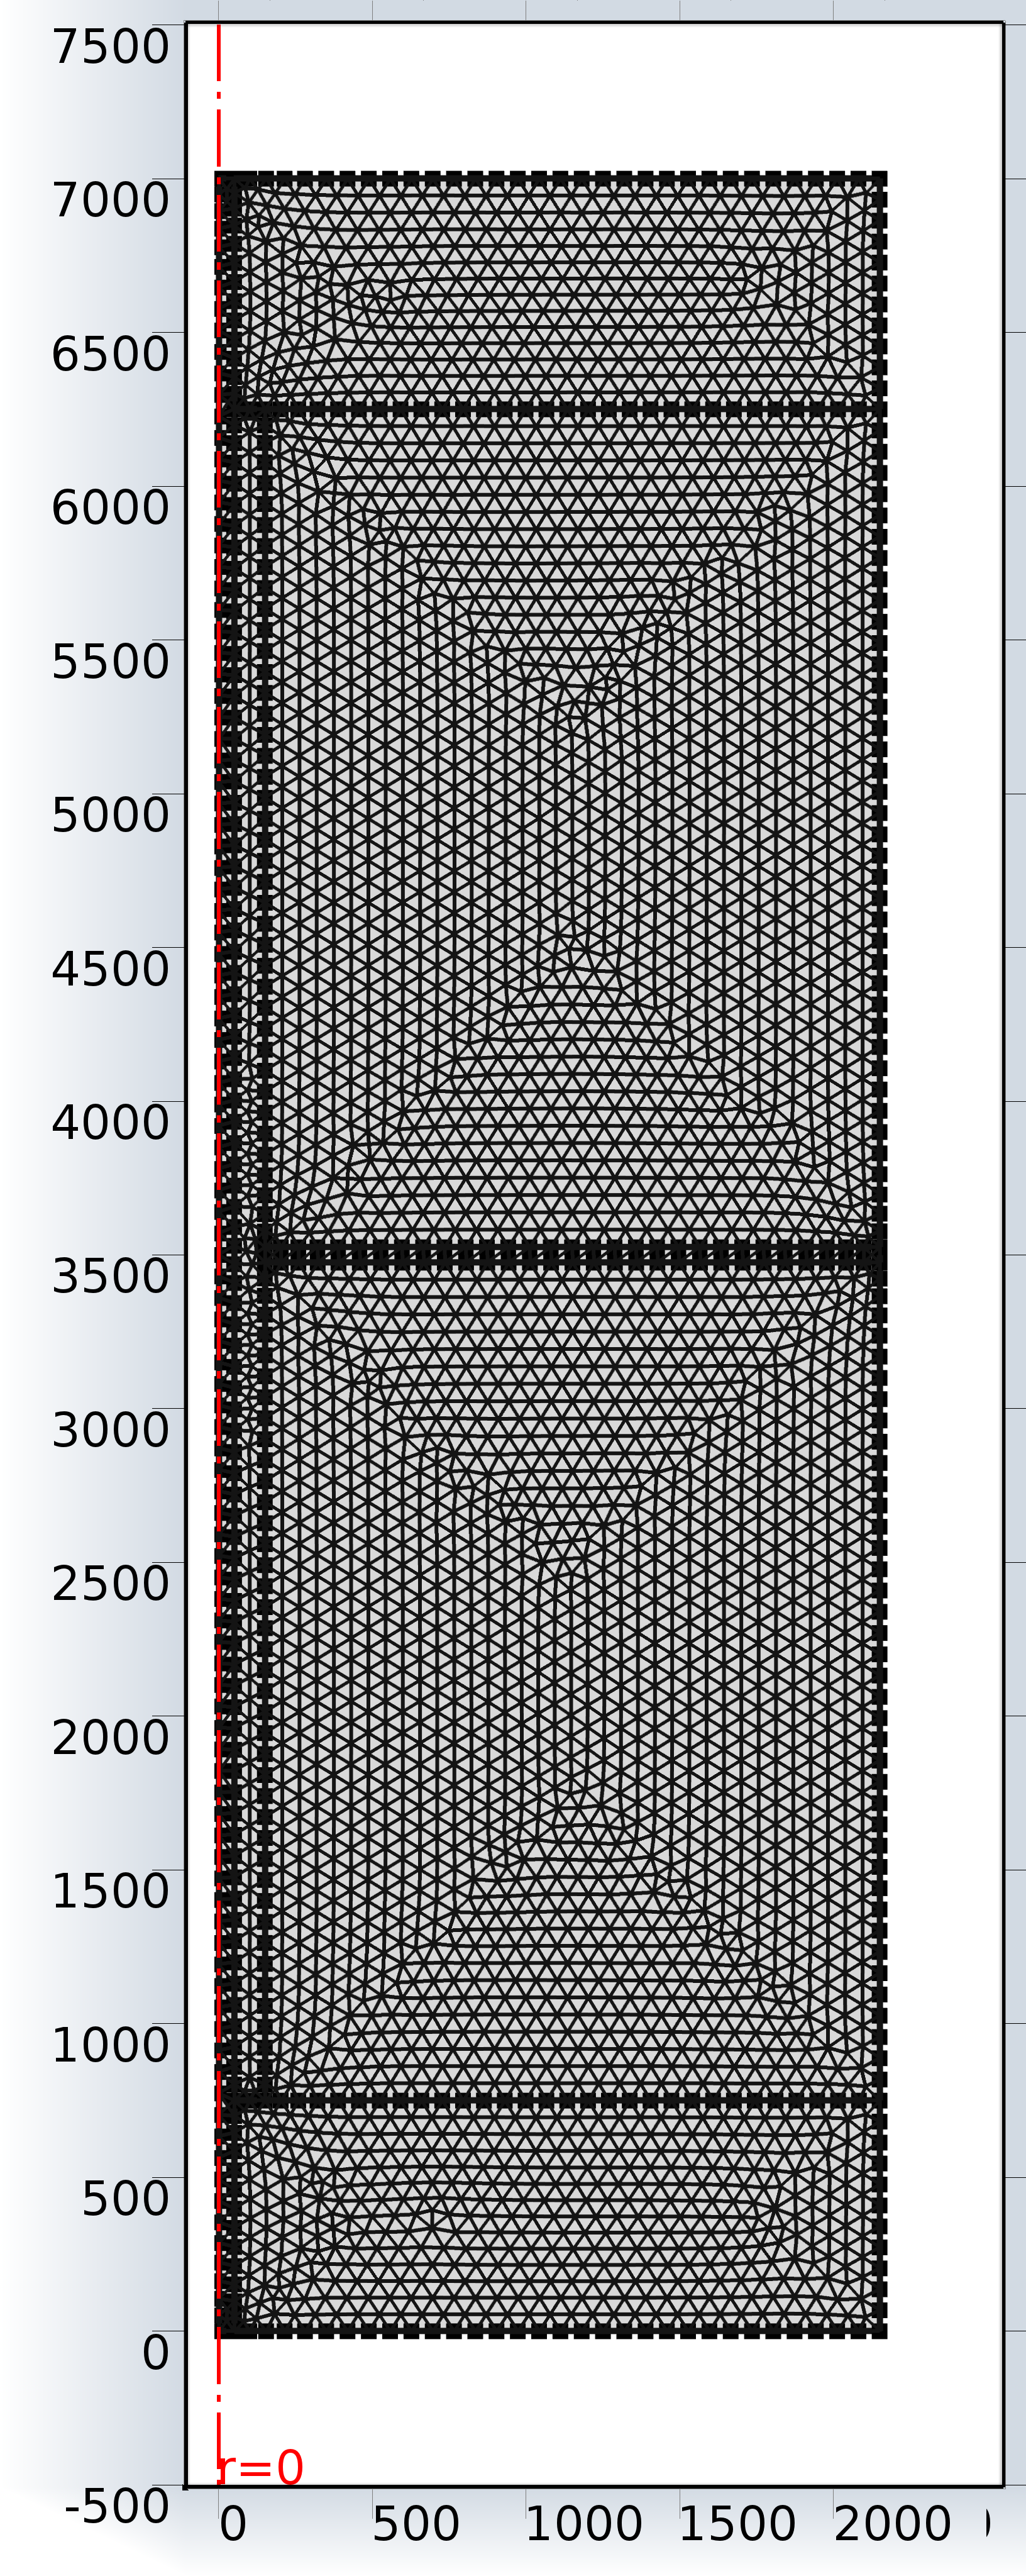
\includegraphics[height = 10cm]{./Figures/Simulations/Edited_No_Foils_Large/Meshing.png} 
	\label{Figure:No_Foil_Large_Mesh}
  }
\subfigure[Normal Electric Field (V/m)]{
    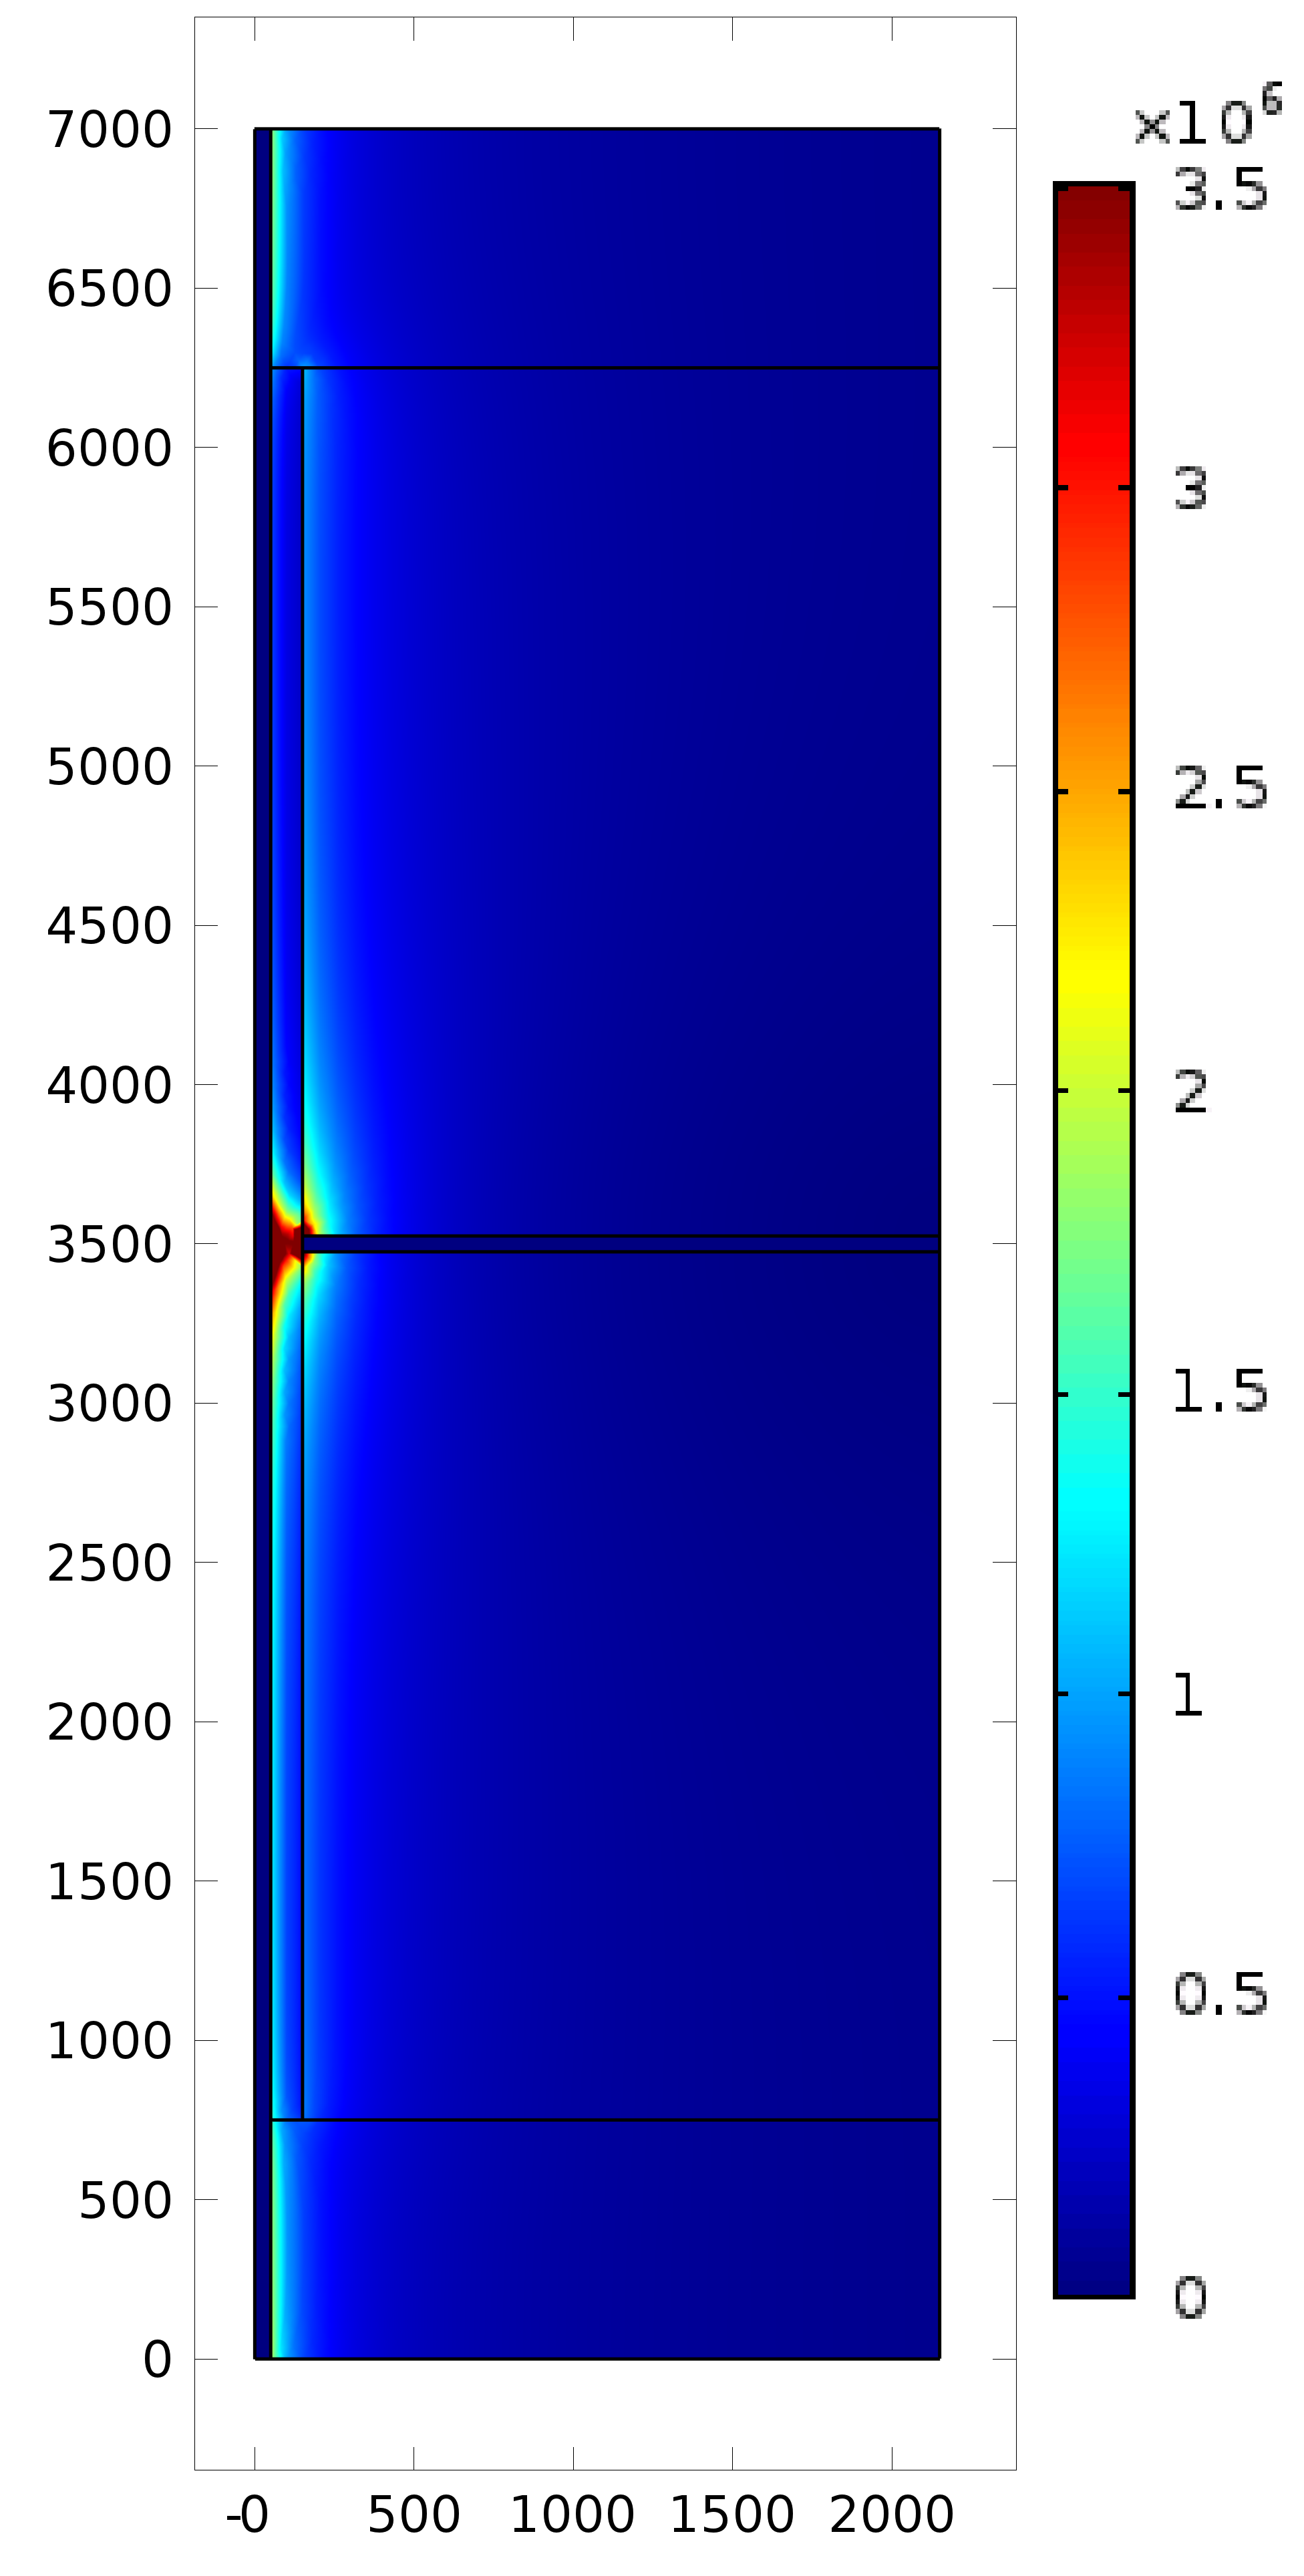
\includegraphics[height = 10cm]{./Figures/Simulations/Edited_No_Foils_Large/Norm_E_Field.png} 
	\label{Figure:No_Foil_Large_Field}
  }
\caption{Baseline Model Simulation - X and Y axis are dimensions in mm}
  \label{Figure:No_Foil_Large}
\end{figure}

The model is made up with a very large geometry. 
The air and oil extends radially 2m from the end of the bushing and 1m in the axial direction.
This is to understand the anticipated area of interest in the model.
By considering figure \ref{Figure:No_Foil_Large_Field} it is clear that there is very little happening further than 500mm radially from the bushing surface and there is very little of interest further than 200mm in the radial direction.
Therefore all further models will adhere to this geometry, ensuring that the area of interest is captured, while decreasing simulation times to a minimum.

\subsection{No Foils}
\dots

\subsection{No Grading}
\dots

\subsection{Radial Grading}
\dots

\subsection{Axial Grading}
\dots
 

%\subsection{No Grading}
%As a baseline for comparison, a bushing with no foils has been constructed and simulated.
%The geometry of the model was built as in figure \ref{figure:Geom:Nograde}.
%The system is an axialsymmetric 2D model, which takes the central vertical point $r=0$ as the centre of a cylinder.
%\begin{figure}[!h]
%   \centering
%   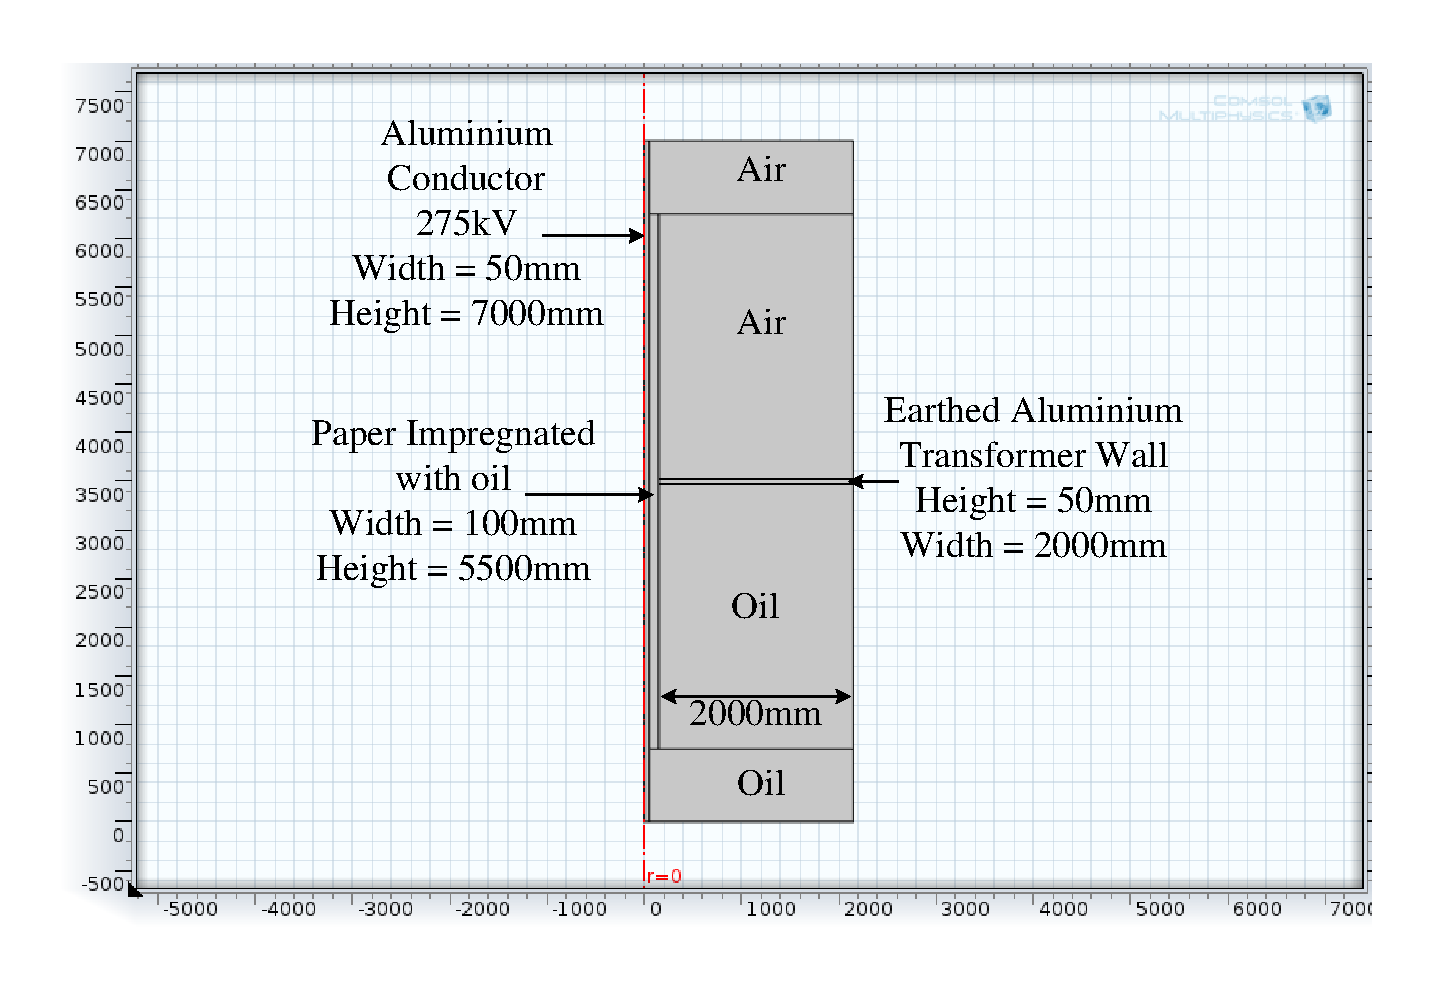
\includegraphics[width = 0.8\textwidth]{NoGradingBlock.pdf}
%   \caption{COMSOL Geometry Annotated with Materials - No Grading}
%   \label{figure:Geom:Nograde}
%\end{figure}
%
%Once the geometry of the model is defined, a finite element mesh can be created as shown in figure \ref{figure:Mesh:Nograde}.
%This model is fairly simple, hence a very fine graded mesh was used improving the accuracy of results.
%\begin{figure}[!h]
%   \centering
%   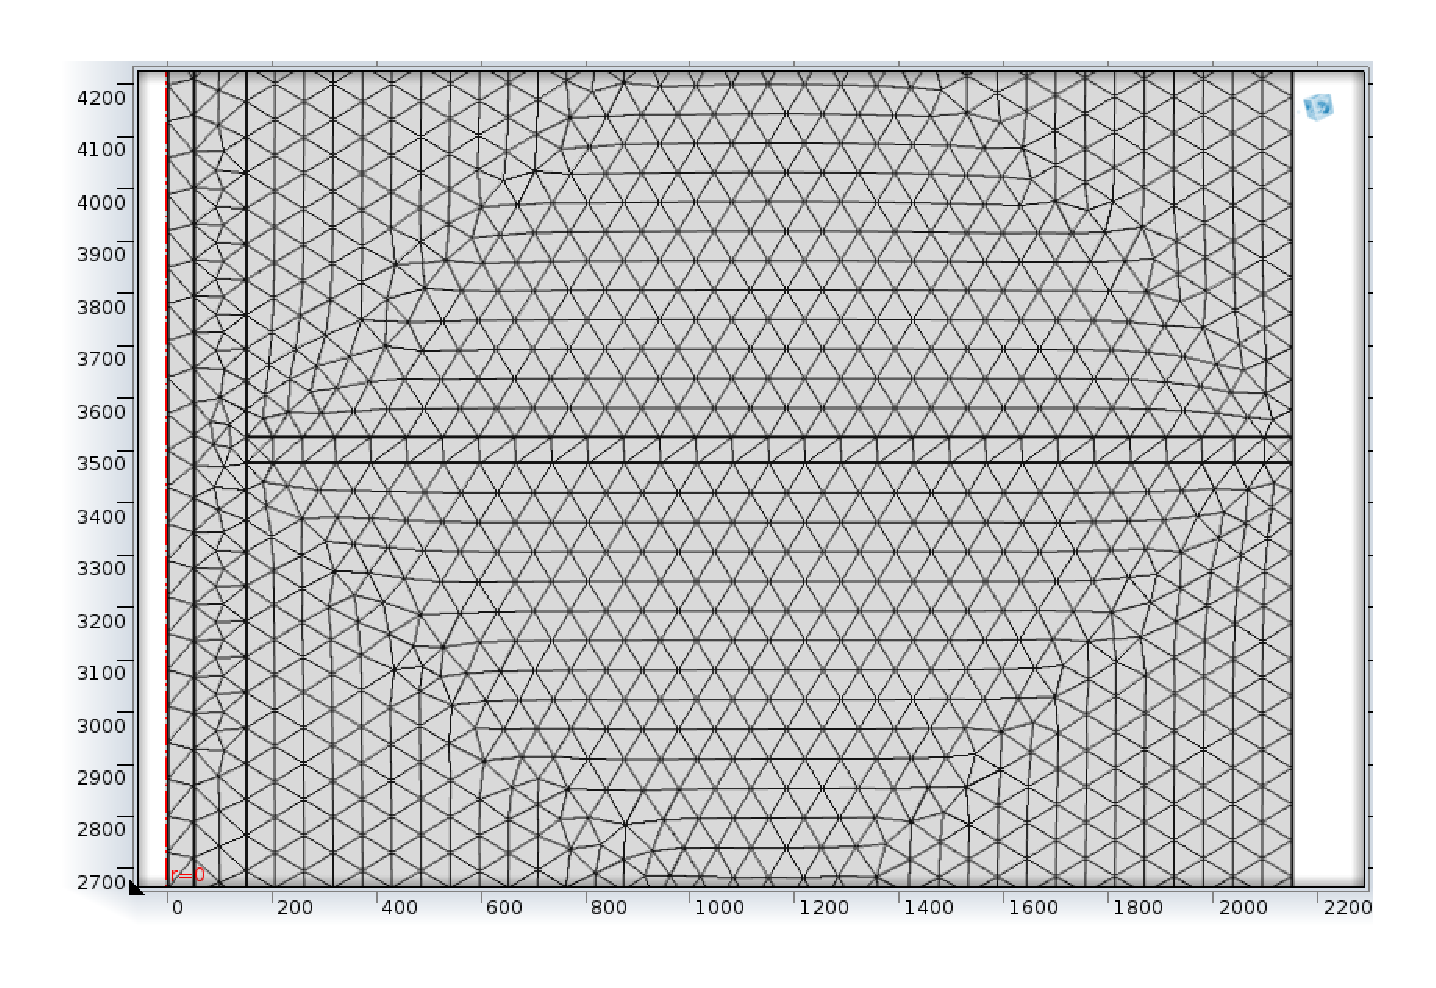
\includegraphics[width = 0.8\textwidth]{NoGradingMesh.pdf}
%   \caption{COMSOL Mesh - No Grading}
%   \label{figure:Mesh:Nograde}
%\end{figure}
%
%The next stage is to define the relative permittivity of each of the materials used for each sub section of the geometry.
%The initial conditions must then be set, with the conductor set to 275kV, and the transformer wall and all outer boundaries earthed.
%All other boundaries are assumed to be continuity boundaries.
%
%The model can then be solved to give the electric field distribution
%\inote{TS - Report done up to here 03/03/2014}
.
%\begin{figure}[!h]
%   \centering
%   \includegraphics[width = 0.8\textwidth]{WideNoGrading.png}
%\end{figure}
%
%\begin{figure}[!h]
%   \centering
%   \includegraphics[width = 0.8\textwidth]{CloseNoGrading.png}
%\end{figure}
%
%\begin{figure}[!h]
%   \centering
%   \includegraphics[width = 0.8\textwidth]{SurfaceGraded21.png}
%\end{figure}
%
%\begin{figure}[!h]
%   \centering
%   \includegraphics[width = 0.8\textwidth]{WideGraded21.png}
%\end{figure}
%
%\begin{figure}[!h]
%   \centering
%   \includegraphics[width = 0.8\textwidth]{CloseGraded21.png}
%\end{figure}
%
%\begin{figure}[!h]
%   \centering
%   \includegraphics[width = 0.8\textwidth]{SurfaceGradedCloseish21.png}
%\end{figure}